\documentclass[10pt,letterpaper]{book}
\usepackage[utf8]{inputenc}
\usepackage[spanish]{babel}
\usepackage{amsmath}
\usepackage{amsfonts}
\usepackage{amssymb}
\usepackage{graphicx}
\usepackage{empheq}
\usepackage{svg}
\usepackage{hyperref}
\usepackage{hypcap}
\usepackage[spanish,onelanguage,linesnumbered,ruled,vlined]{algorithm2e}
\usepackage{titling}
\pretitle{%
  \begin{flushright}
  \vspace{-10cm}
%  
\includegraphics[width=5cm,natwidth=472,natheight=531]{logo} \\[7cm]
  
\includegraphics[width=5cm]{logo} \\[6cm]
  \end{flushright}
  \begin{center}
  \LARGE
}
\posttitle{\end{center}}
\usepackage[left=3cm,right=2.5cm,top=3cm,bottom=2.5cm,includehead,includefoot,headheight=15pt]{geometry}
\usepackage{setspace}
\setstretch{0.99}
\usepackage{fancyhdr}
%\date{27 de Noviembre 2018}
\fancyhf{}
\renewcommand{\headrulewidth}{0pt} % optional
%\fancyhead[L]{\nouppercase{\leftmark} \hfill Section \nouppercase{\rightmark}}
\fancyhead[L]{Método Simplex}
\cfoot{\thepage}
\pagestyle{fancy}
\author{
Leonardo Henry Añez Vladimirovna\\
\texttt{Reg: 217002498}
\and
Sebastián Durán\\
\texttt{Reg: 217050662}
}
\title{
Investigación Operativa I (MAT329)\\ ${ }$\\
\textbf{Aplicación del Método Simplex en la Panadería: ''Barrio Lindo''}
\\ ${ }$\\
\small Facultad de Ingeniería en Ciencias de la Computación y Telecomunicaciones\\}

\graphicspath{ {./images/} }
\begin{document}
\maketitle
\section*{Problema}
En este trabajo se plantea utilizar el Método Simplex en la resolución de un problema de Programación Lineal. Para realizar el analisis de producción de panes en la Panadería \textit{''Barrio Lindo''}. Buscando la minimización de los costos de produccion basados en un lote de una arroba para distintos tipos de panes.
\section*{Información Técnica}
Contamos con el precio unitario de los ingredientes representativos usados para preparar diferentes panes, esto para un lote.
\begin{center}
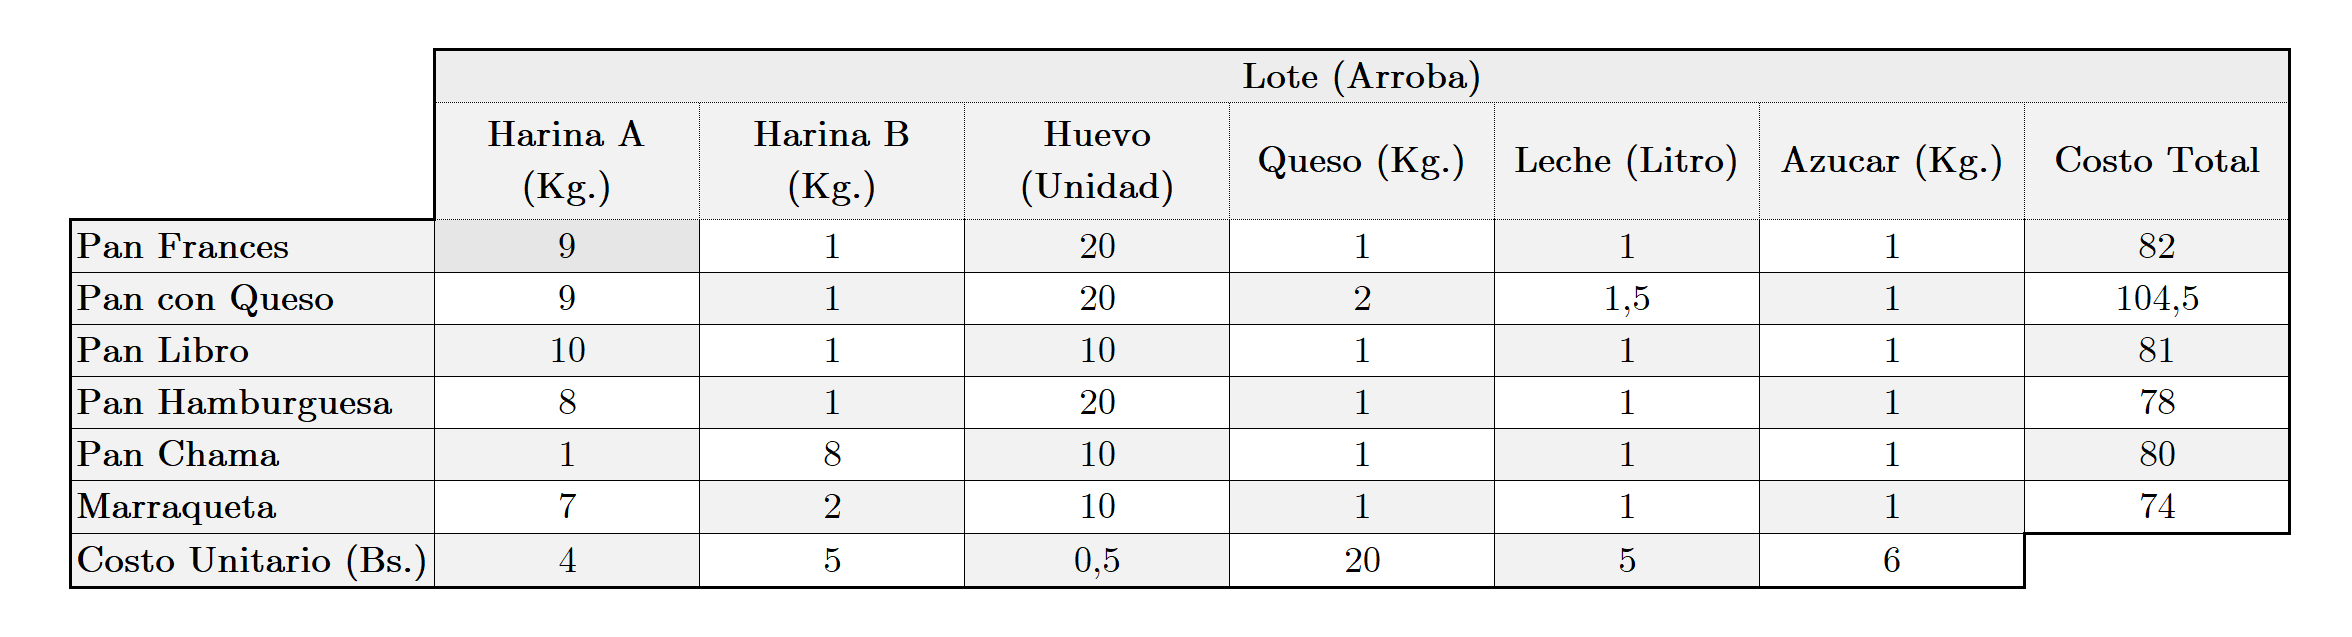
\includegraphics[scale=0.66]{Tabla}
\end{center}
Además de contar con cierta disponibilidad por cada ingrediente:
\begin{center}
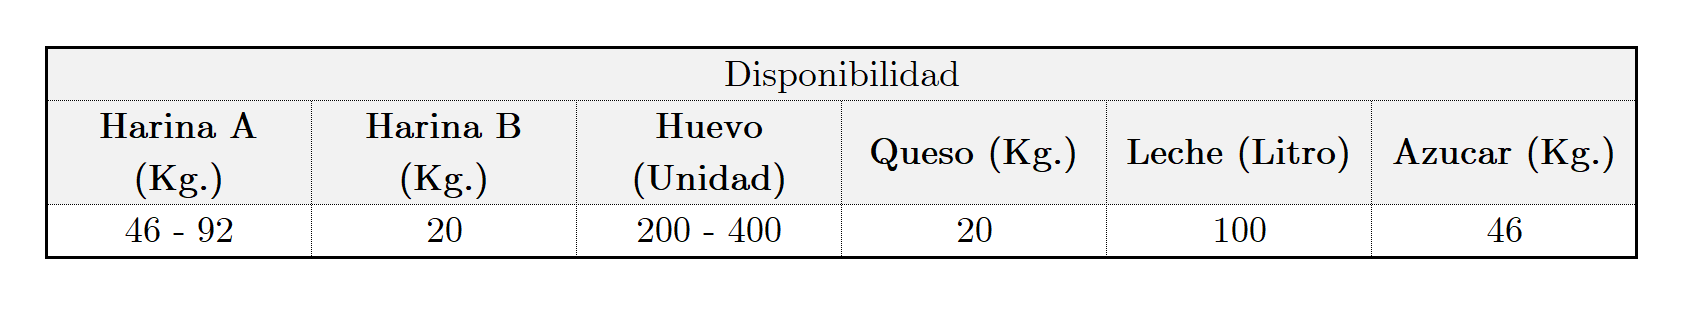
\includegraphics[scale=0.66]{Tabla2}
\end{center}
\section*{Modelo Matemático}
El modelo matemático tendra el siguiente esquema:
\subsection*{Variables}
Las variables del trabajo serán las cantidades por tipos de pan que se venden y estarán representados por:
\begin{align*}
x_1,x_2,x_3,x_4,x_5,x_6
\end{align*}
\subsection*{Función Objetivo}
La función objetivo estará dada de la  siguiente manera:
$$
z = 82x_1 + 104.5x_2 + 81x_3 + 78x_4 + 80x_5 + 74x_6
$$
\subsection*{Restricciones}
Las restricciones al problema serán las siguientes:

\begin{align*}
9x_1 + 9x_2 + 10x_3 + 8x_4 + x_5 + 7x_6 &\geq 46 \\
9x_1 + 9x_2 + 10x_3 + 8x_4 + x_5 + 7x_6 &\leq 92 \\
x_1 + x_2 + x_3 + x_4 + 8x_5 + 2x_6 &\leq 20 \\
20x_1 + 20x_2 + 10x_3 + 20x_4 + 10x_5 + 10x_6 &\geq 200 \\
20x_1 + 20x_2 + 10x_3 + 20x_4 + 10x_5 + 10x_6 &\leq 400 \\
x_1 + 2x_2 + x_3 + x_4 + x_5 + x_6 &\leq 20 \\
x_1 +1.5x_2 + x_3 + x_4 + x_5 + x_6 &\leq 100 \\
x_1 + x_2 + 2x_3 + x_4 + x_5 + x_6 &\leq 46
\end{align*}
\section*{Resultados}
Mediante el uso del programa realizado para el proyecto,procedemos a cargar el programa con las especificaciones necesarias:
\begin{center}
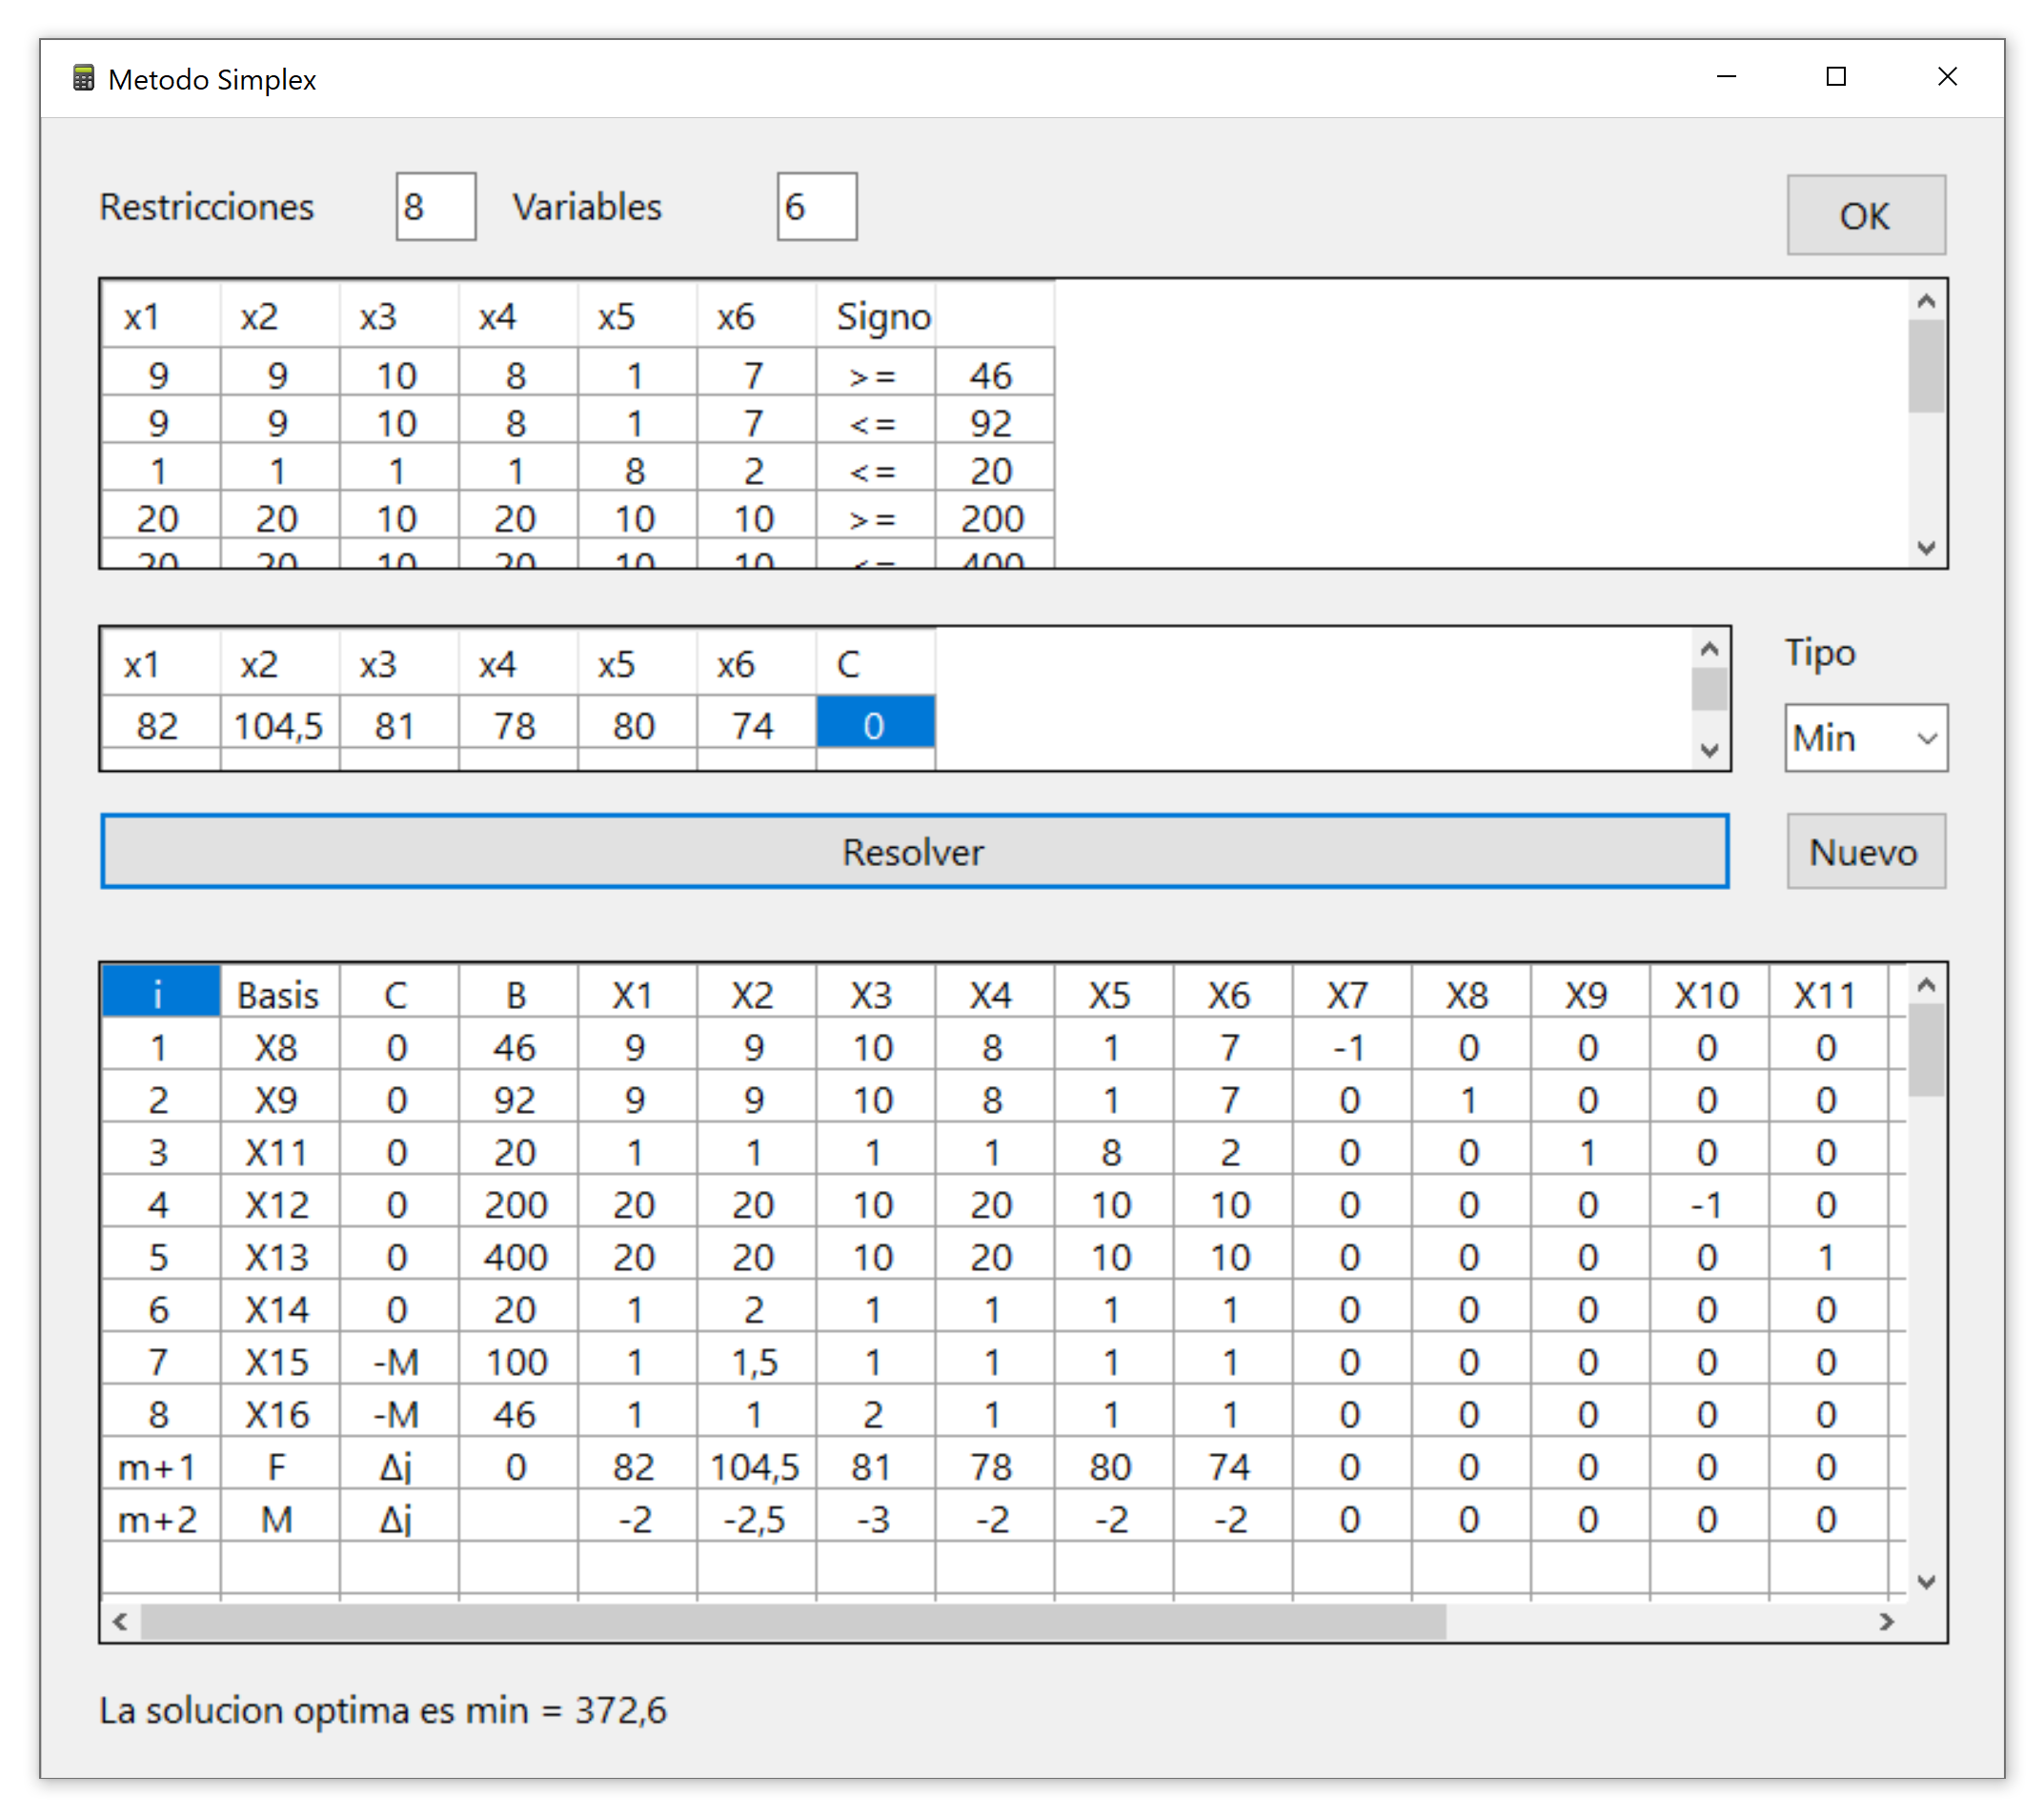
\includegraphics[scale=0.55]{Programa1}
\end{center}
Una vez hacemos click en \texttt{Resolver} nos genera todas las iteraciones hasta llegar a la solución final. \\${ }$\\
\texttt{Iteraciones del Programa}
\begin{center}

\fbox{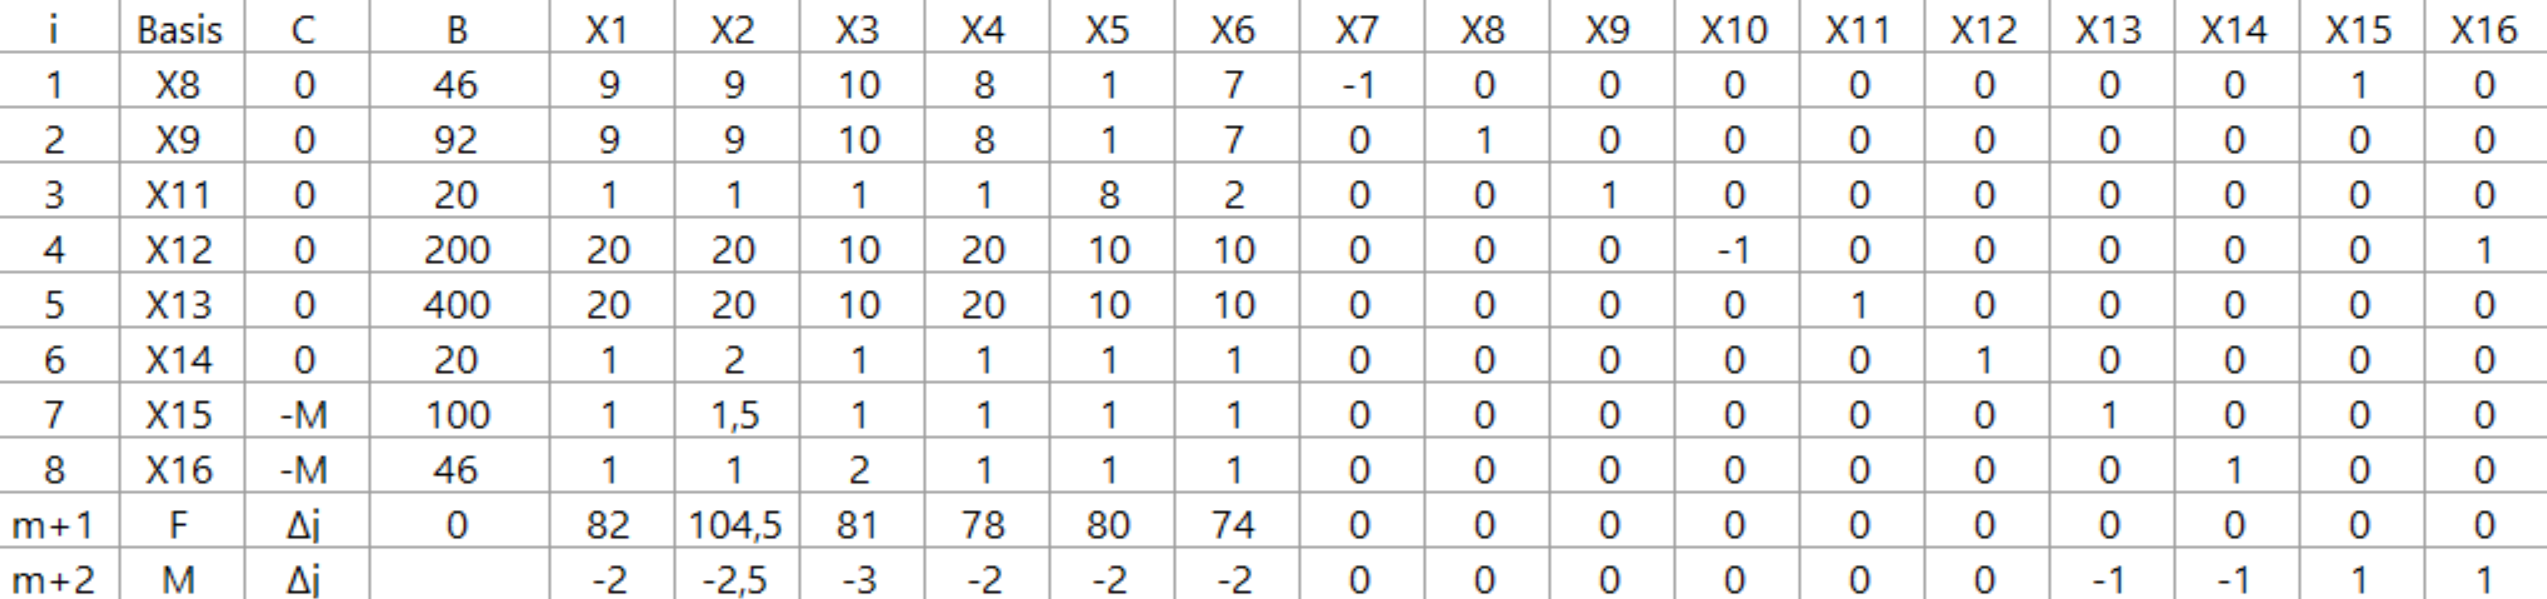
\includegraphics[scale=0.55]{Programa2}}
\fbox{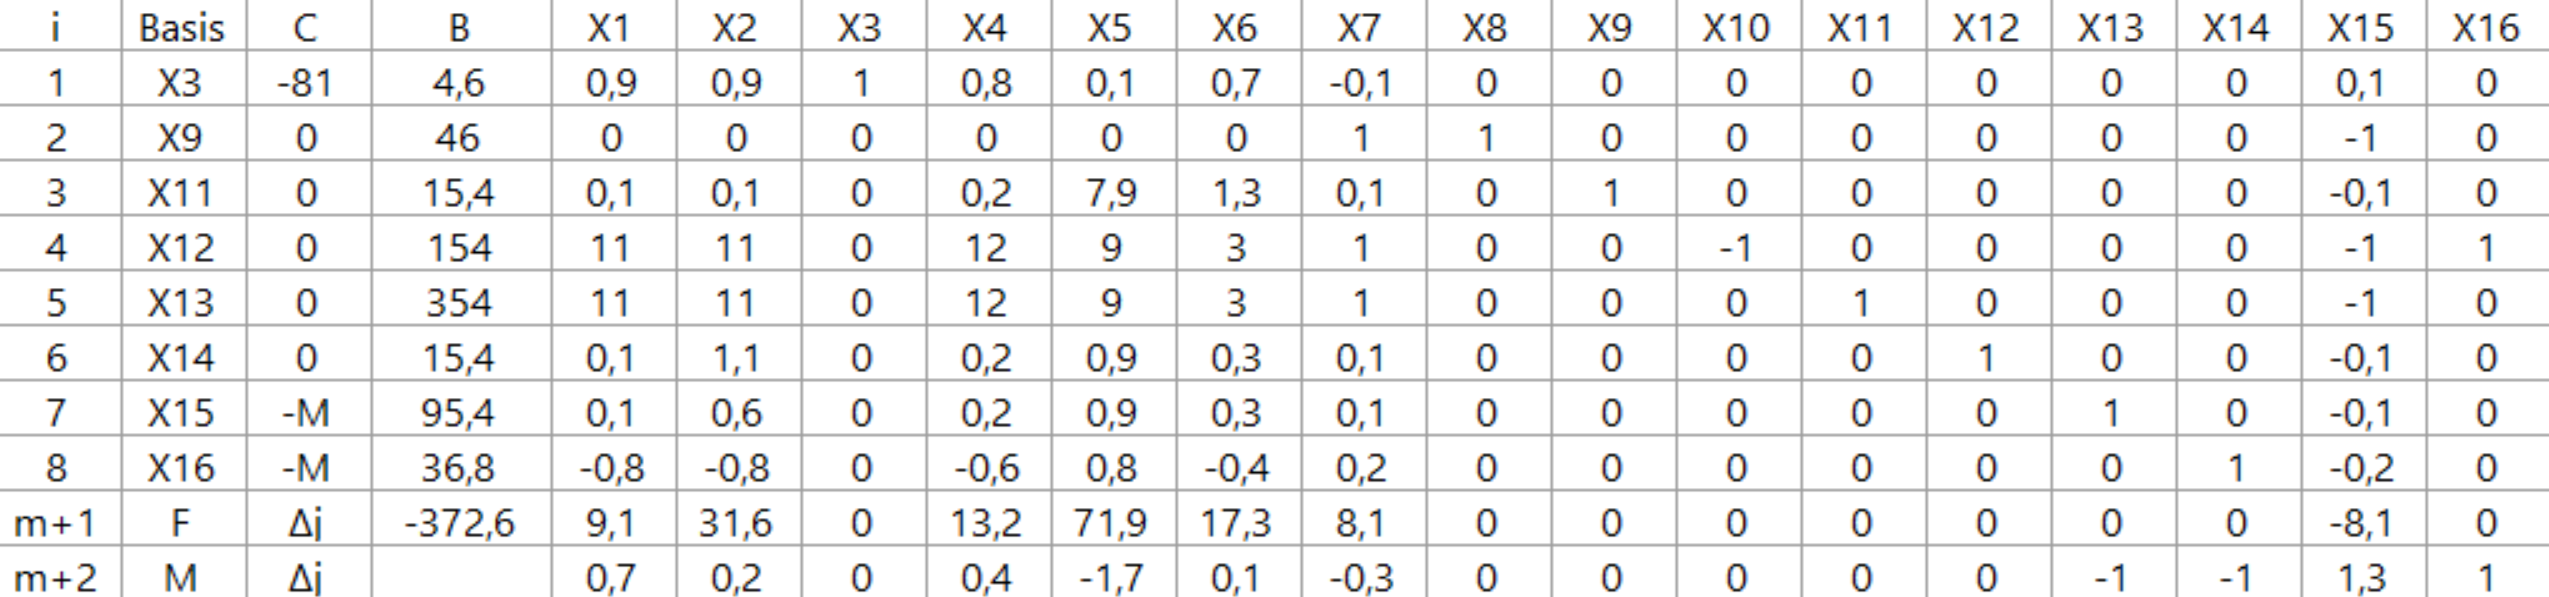
\includegraphics[scale=0.55]{Programa3}}
\fbox{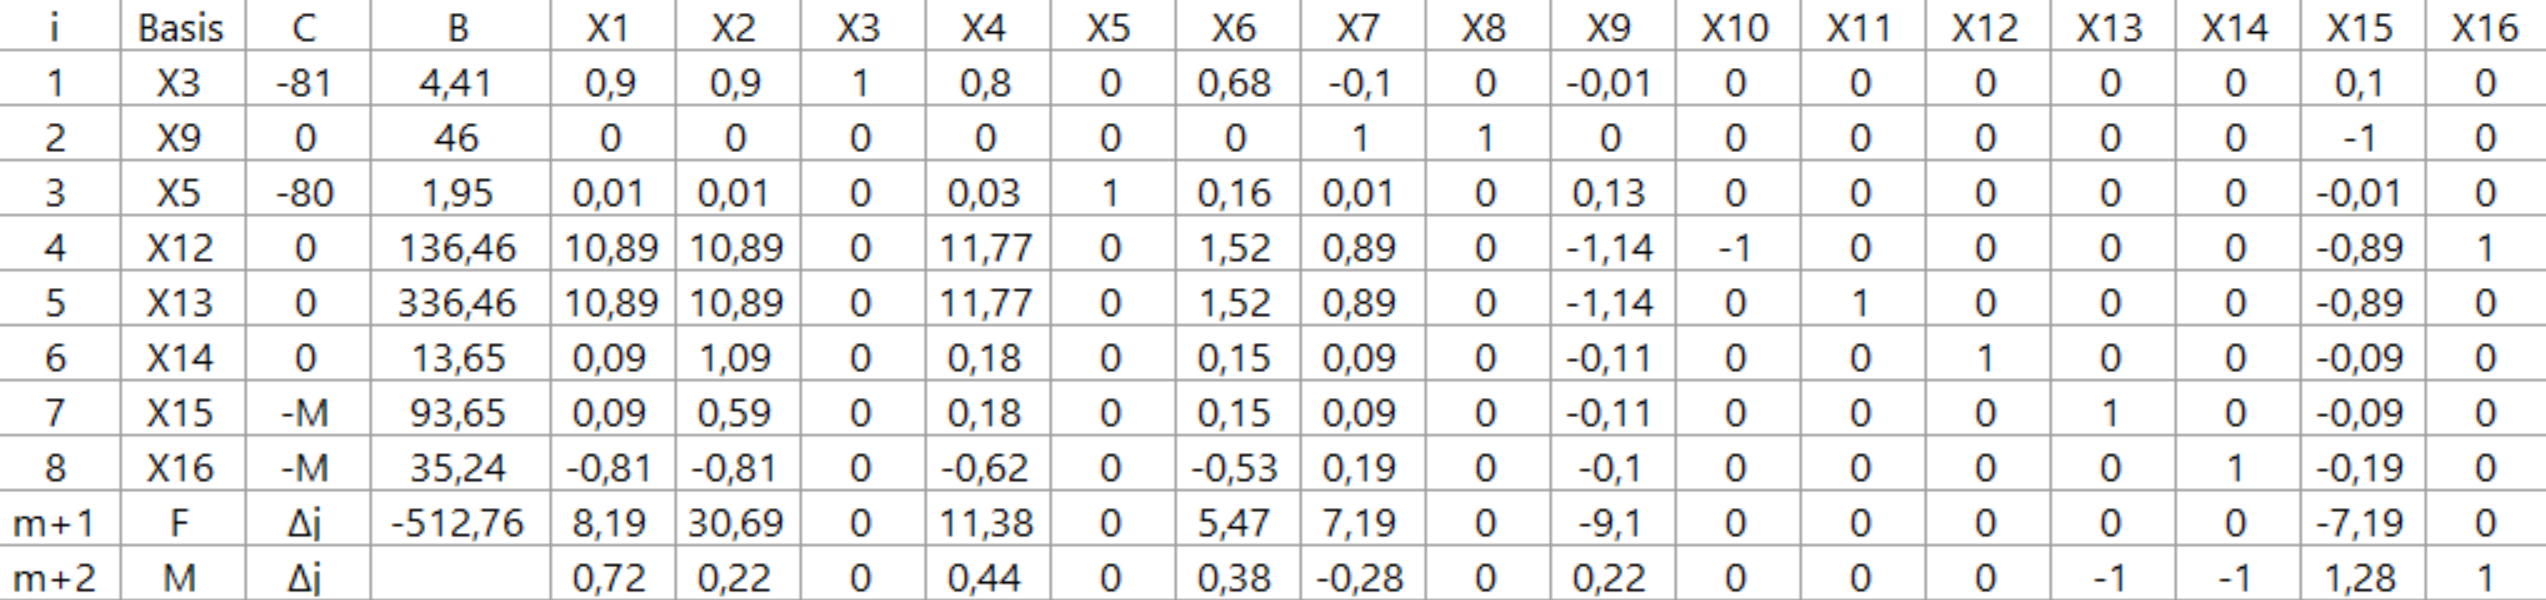
\includegraphics[scale=0.55]{Programa4}}
\fbox{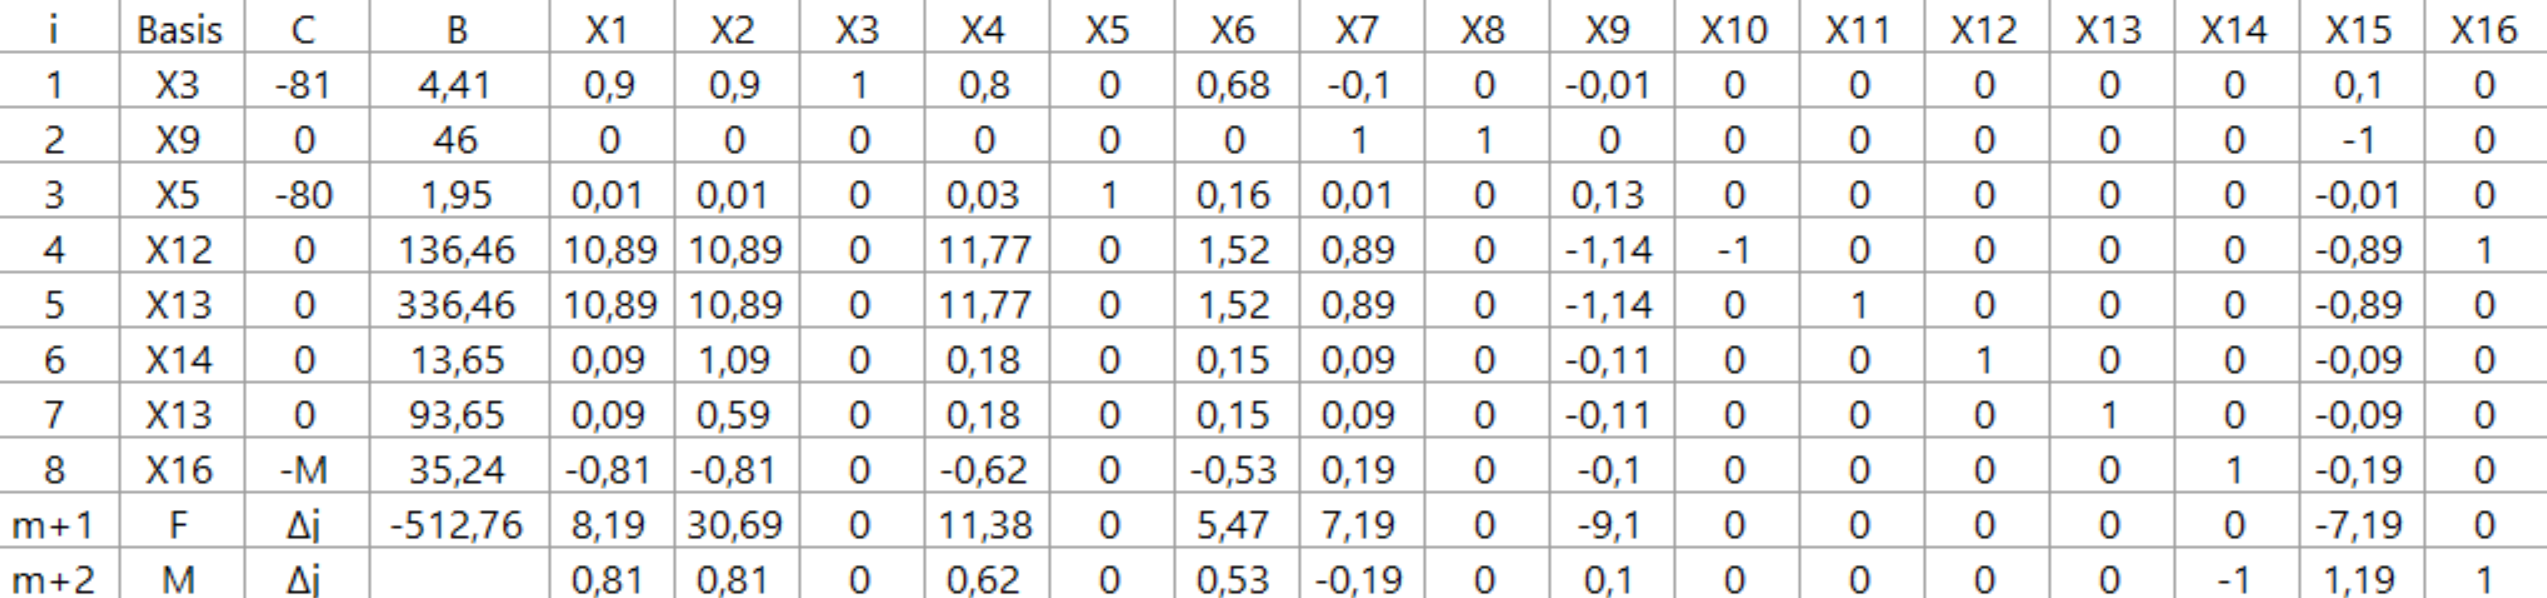
\includegraphics[scale=0.55]{Programa5}}
\fbox{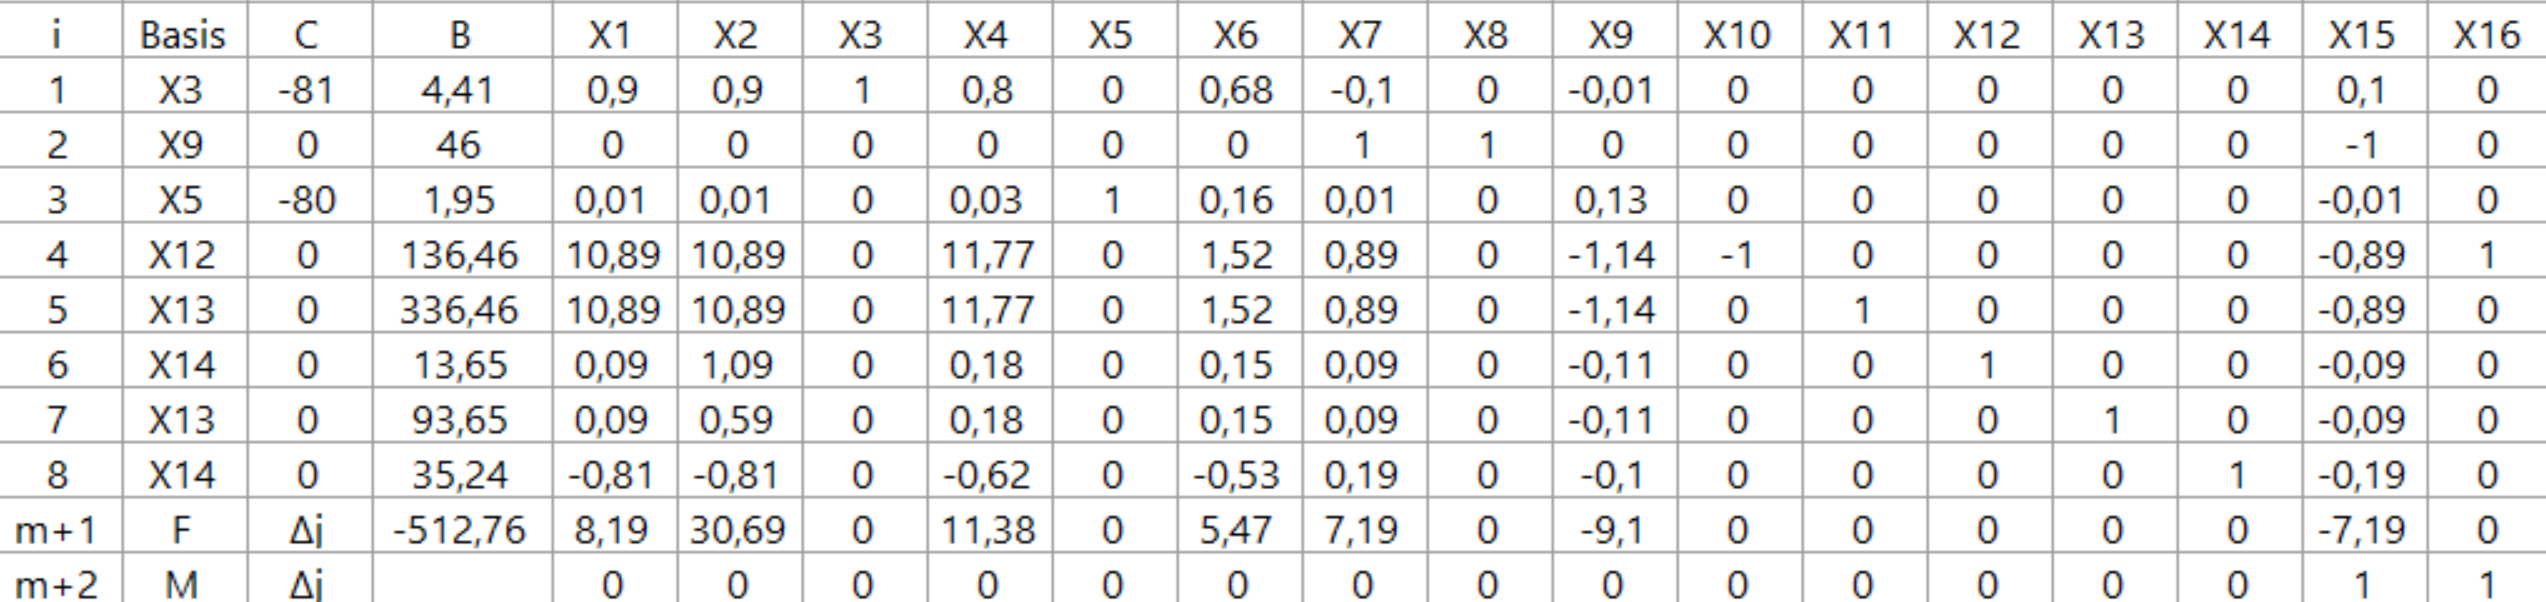
\includegraphics[scale=0.55]{Programa6}}
\end{center}
\pagebreak
Finalmente podemos ver en el programa el resultado final de la minimización.
\begin{center}
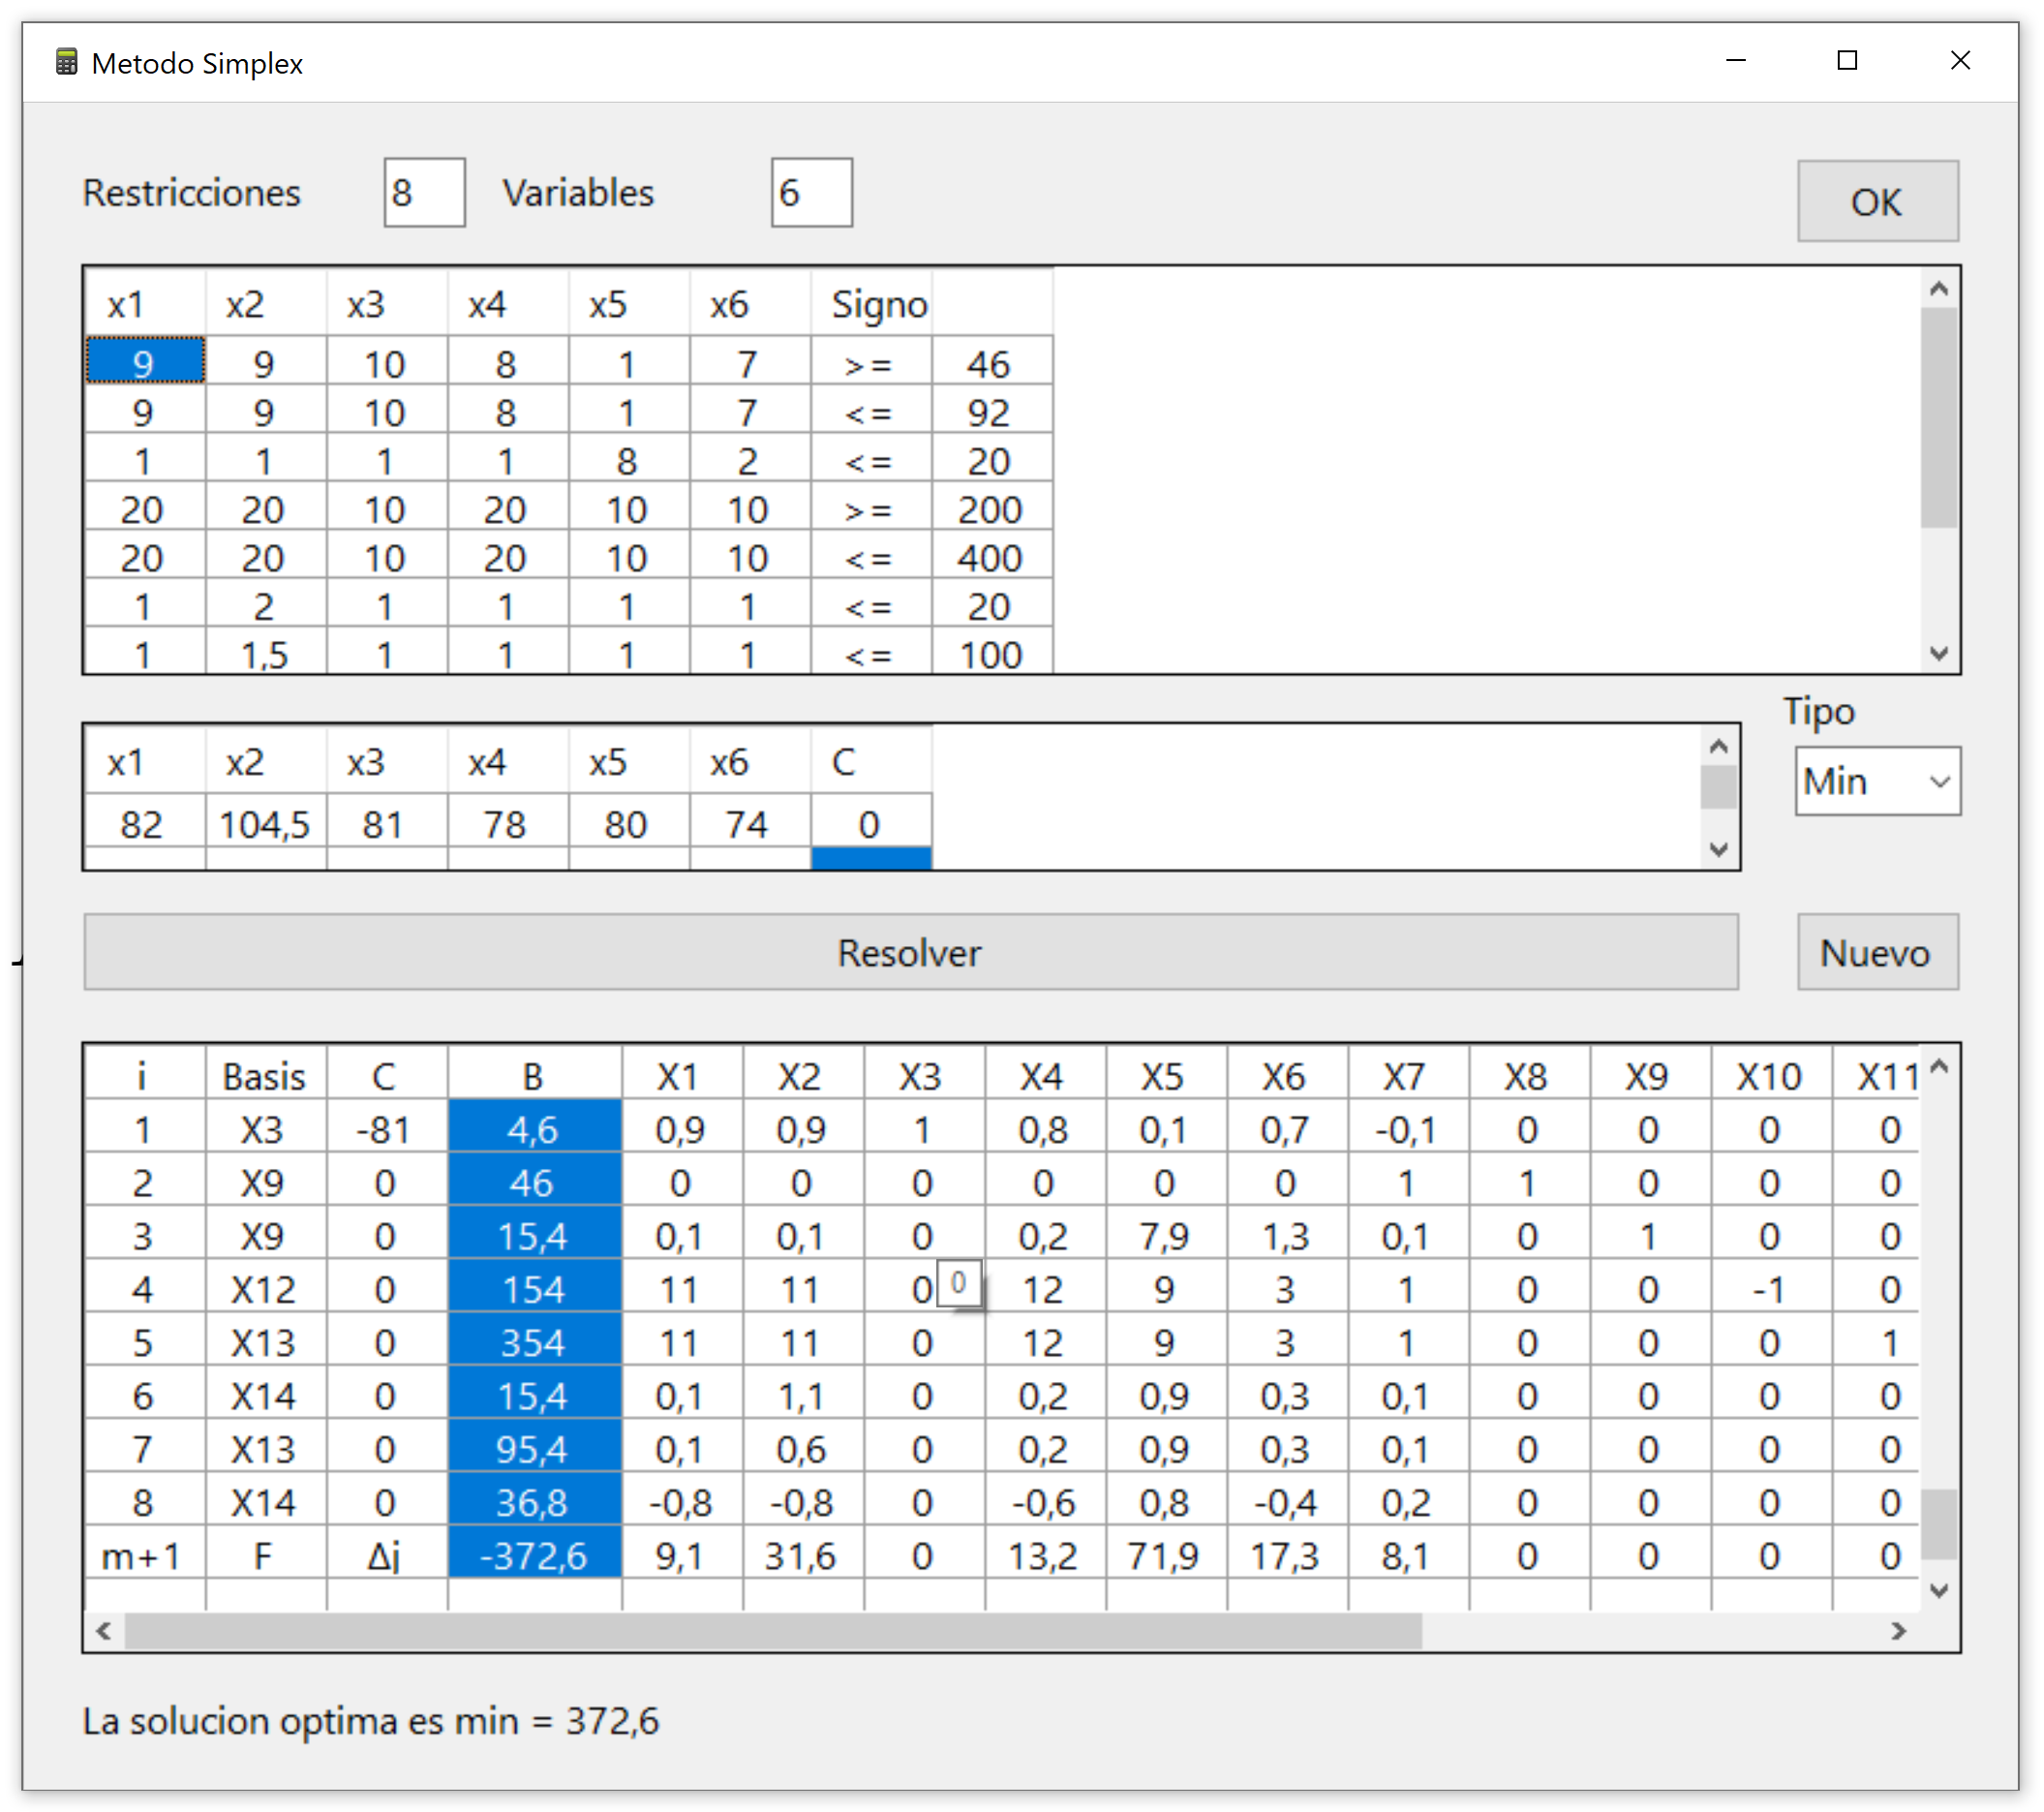
\includegraphics[scale=0.55]{Programa7}
\end{center}
Por lo que tenemos los resultados para la minimizacion de $z$:
\begin{align*}
Min_z &= 372.6 \\ 
x_1   &= 0  \\
x_2   &= 0  \\
x_3   &= 4.6  \\
x_4   &= 0  \\
x_5   &= 0  \\
x_6   &= 0  
\end{align*}

\section*{Conclusión}
\end{document}